\documentclass[]{article}

\usepackage{enumitem}
\usepackage{ulem}

\usepackage{graphicx}
\graphicspath{ {./images/} }

\usepackage{tikz}
\usepackage{tikz-qtree}
\tikzset{every tree node/.style={align=center}}




\title{Lab 1\\CPE 301.1104}
\author{Keaton Clark}

\begin{document}
\maketitle

\section{Setup}
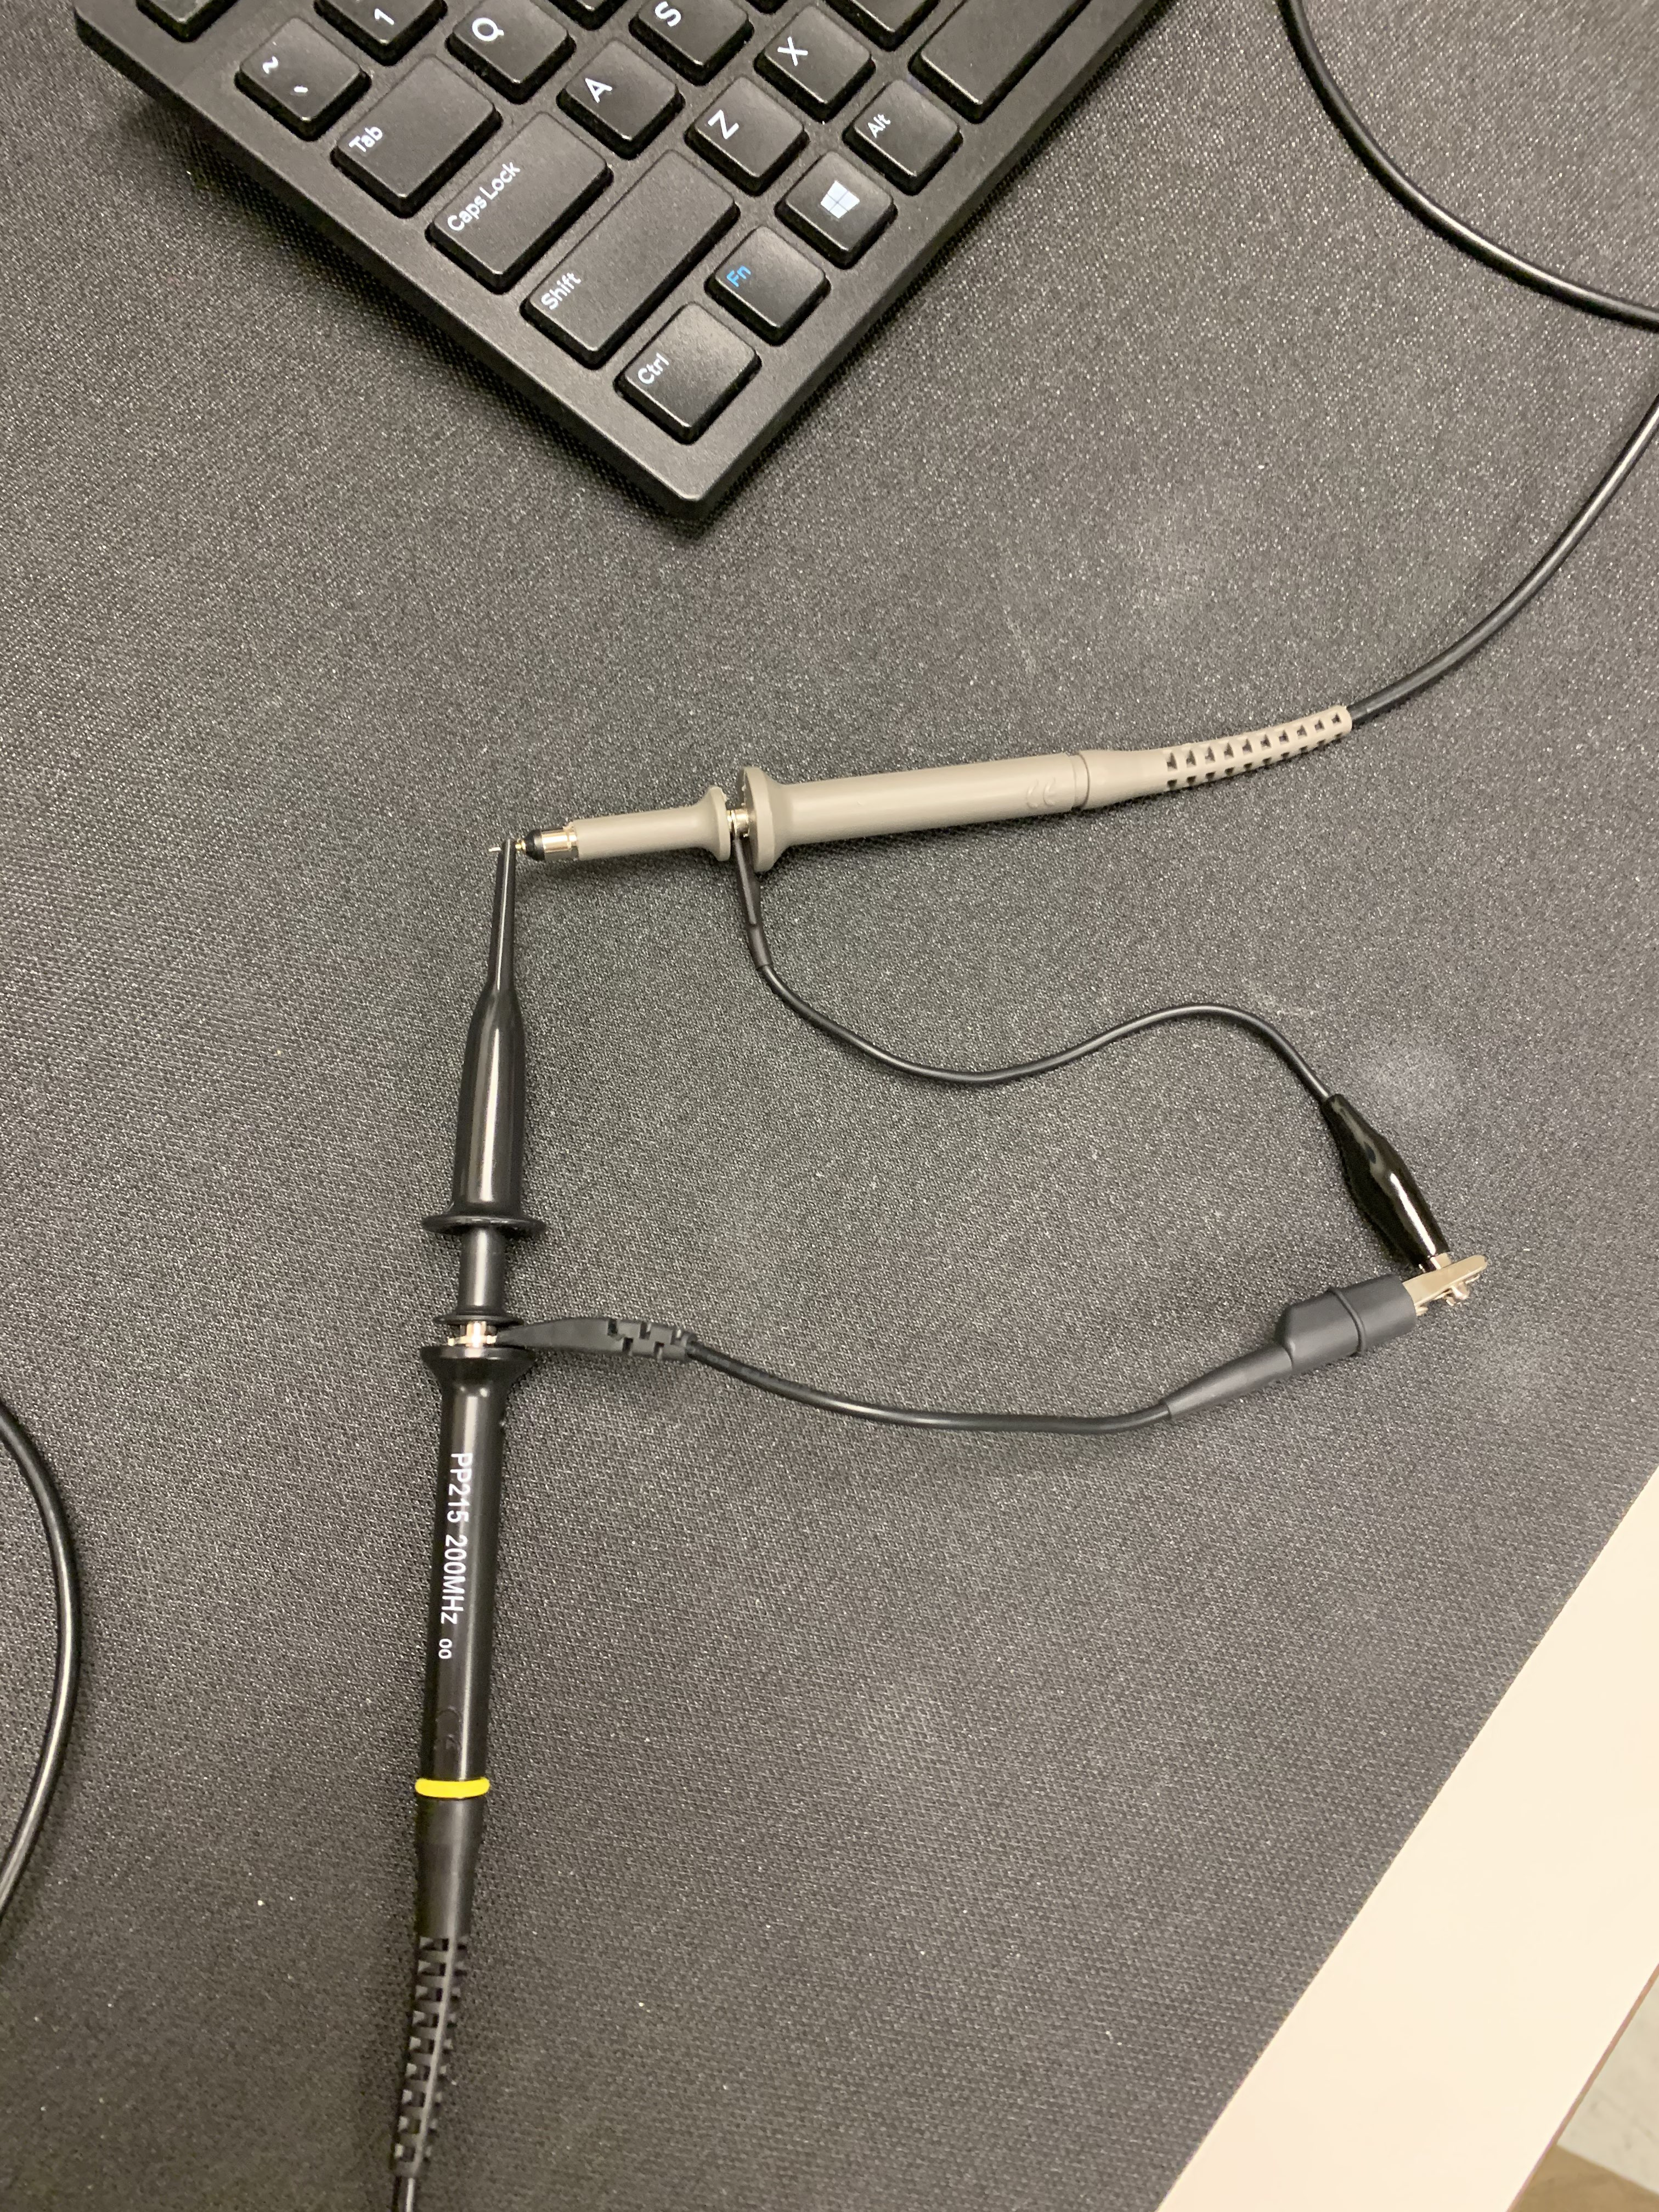
\includegraphics[scale=.1]{connection.jpg}\\
Simply connect the Signal generator to the Oscilloscope with the cable provided to each. Make sure that both provided lines are connected.

\section{Square Wave}
	\begin{center}
		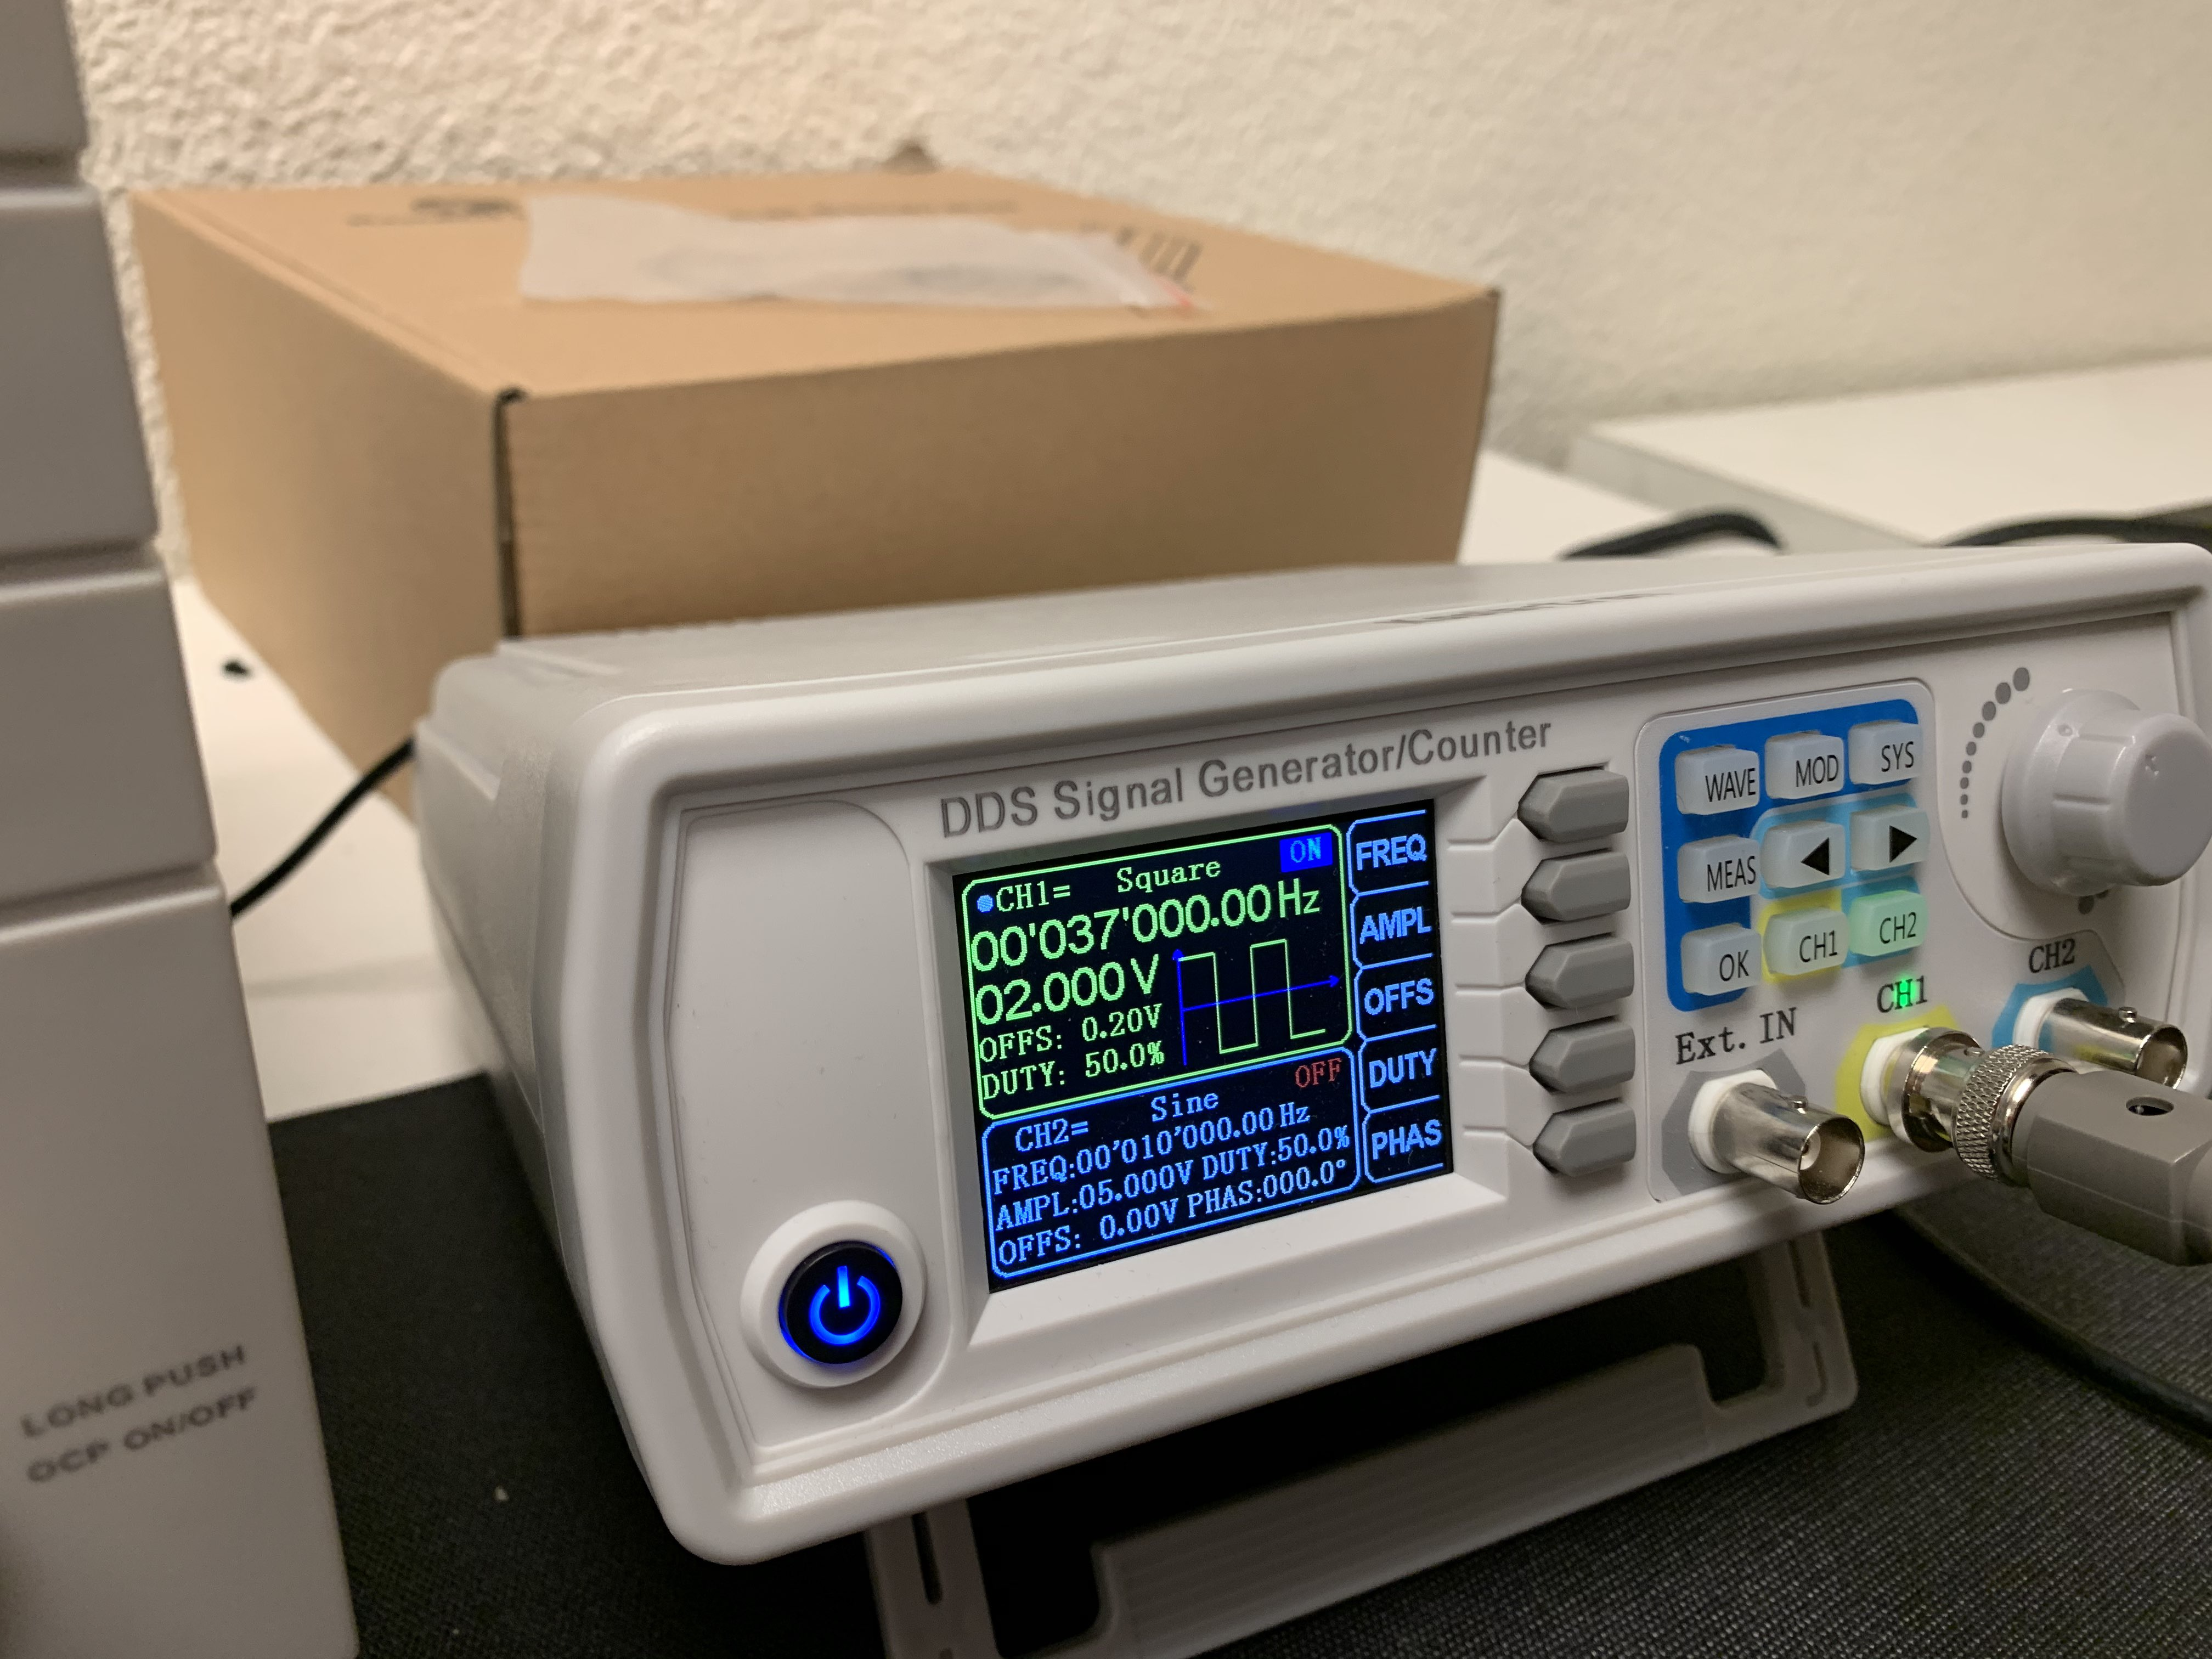
\includegraphics[scale=.05]{square_func.jpg}\\
	\end{center}
	Set up the Signal generator to output a square wave by cycling through the options with the "wave" button.\\

	\begin{center}
		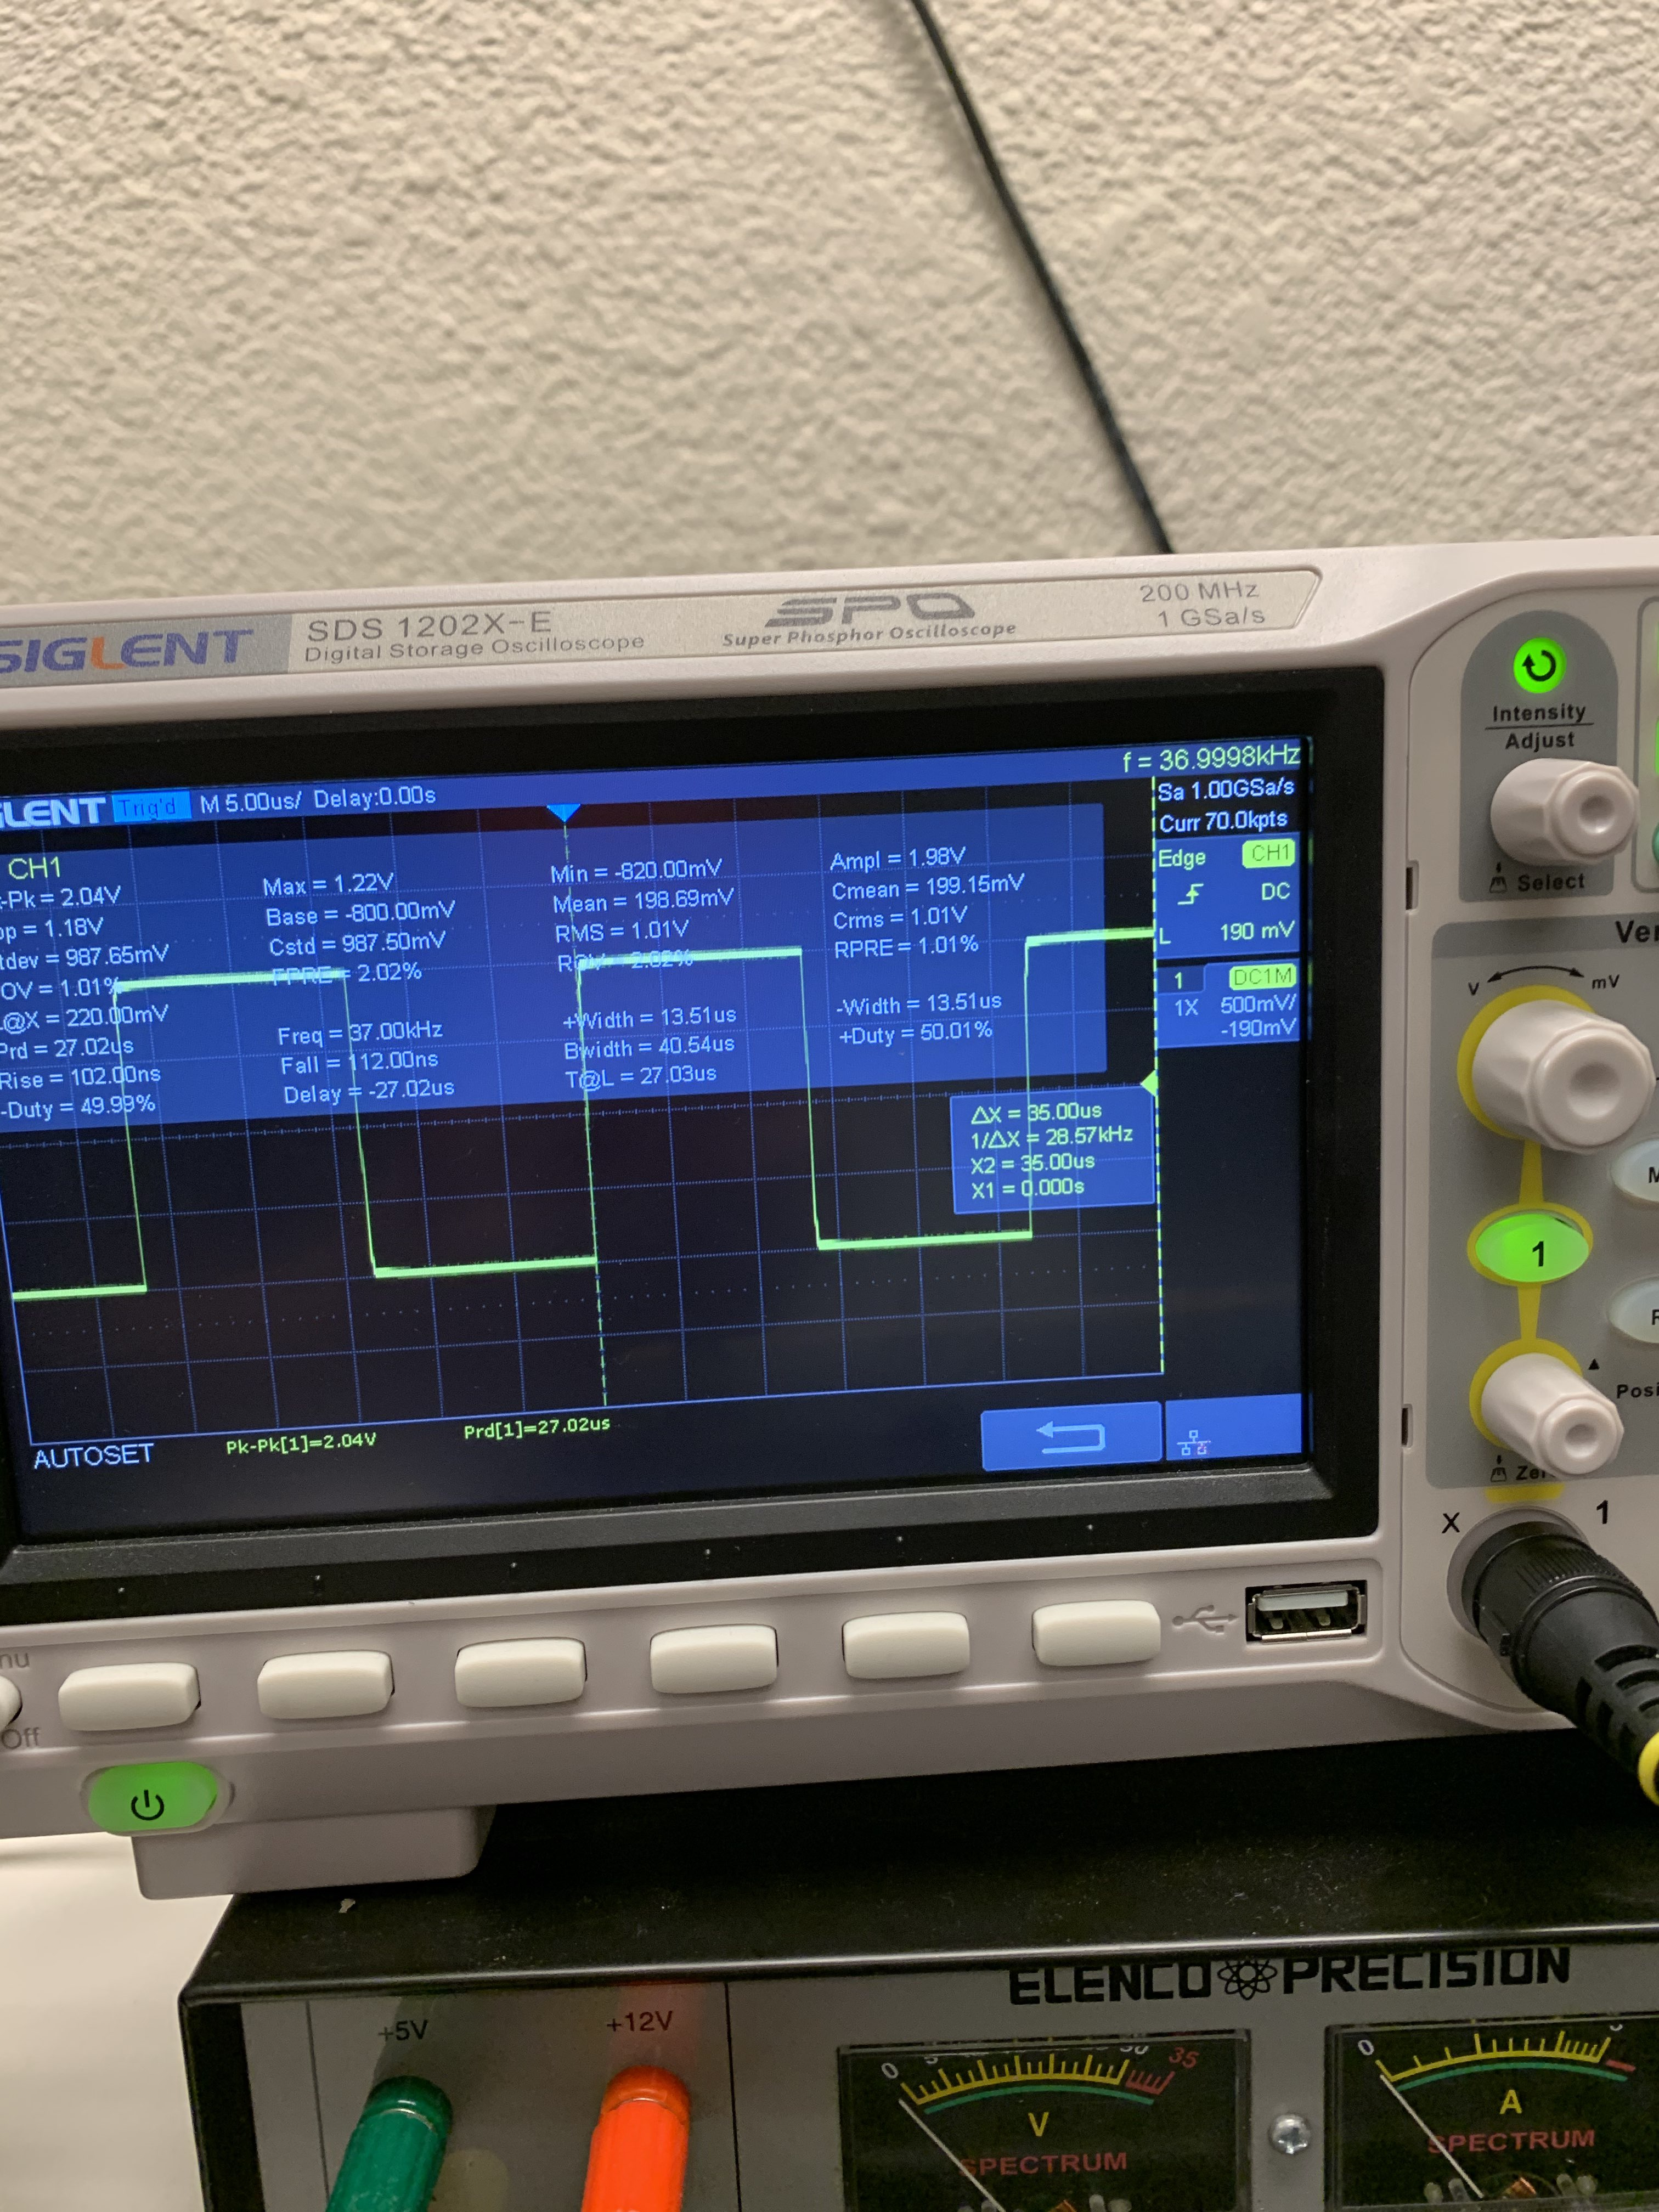
\includegraphics[scale=.05]{square_osci.jpg}\\
	\end{center}
	This is how it appears on the Oscilloscope.

\section{Sin Wave}
	\begin{center}
		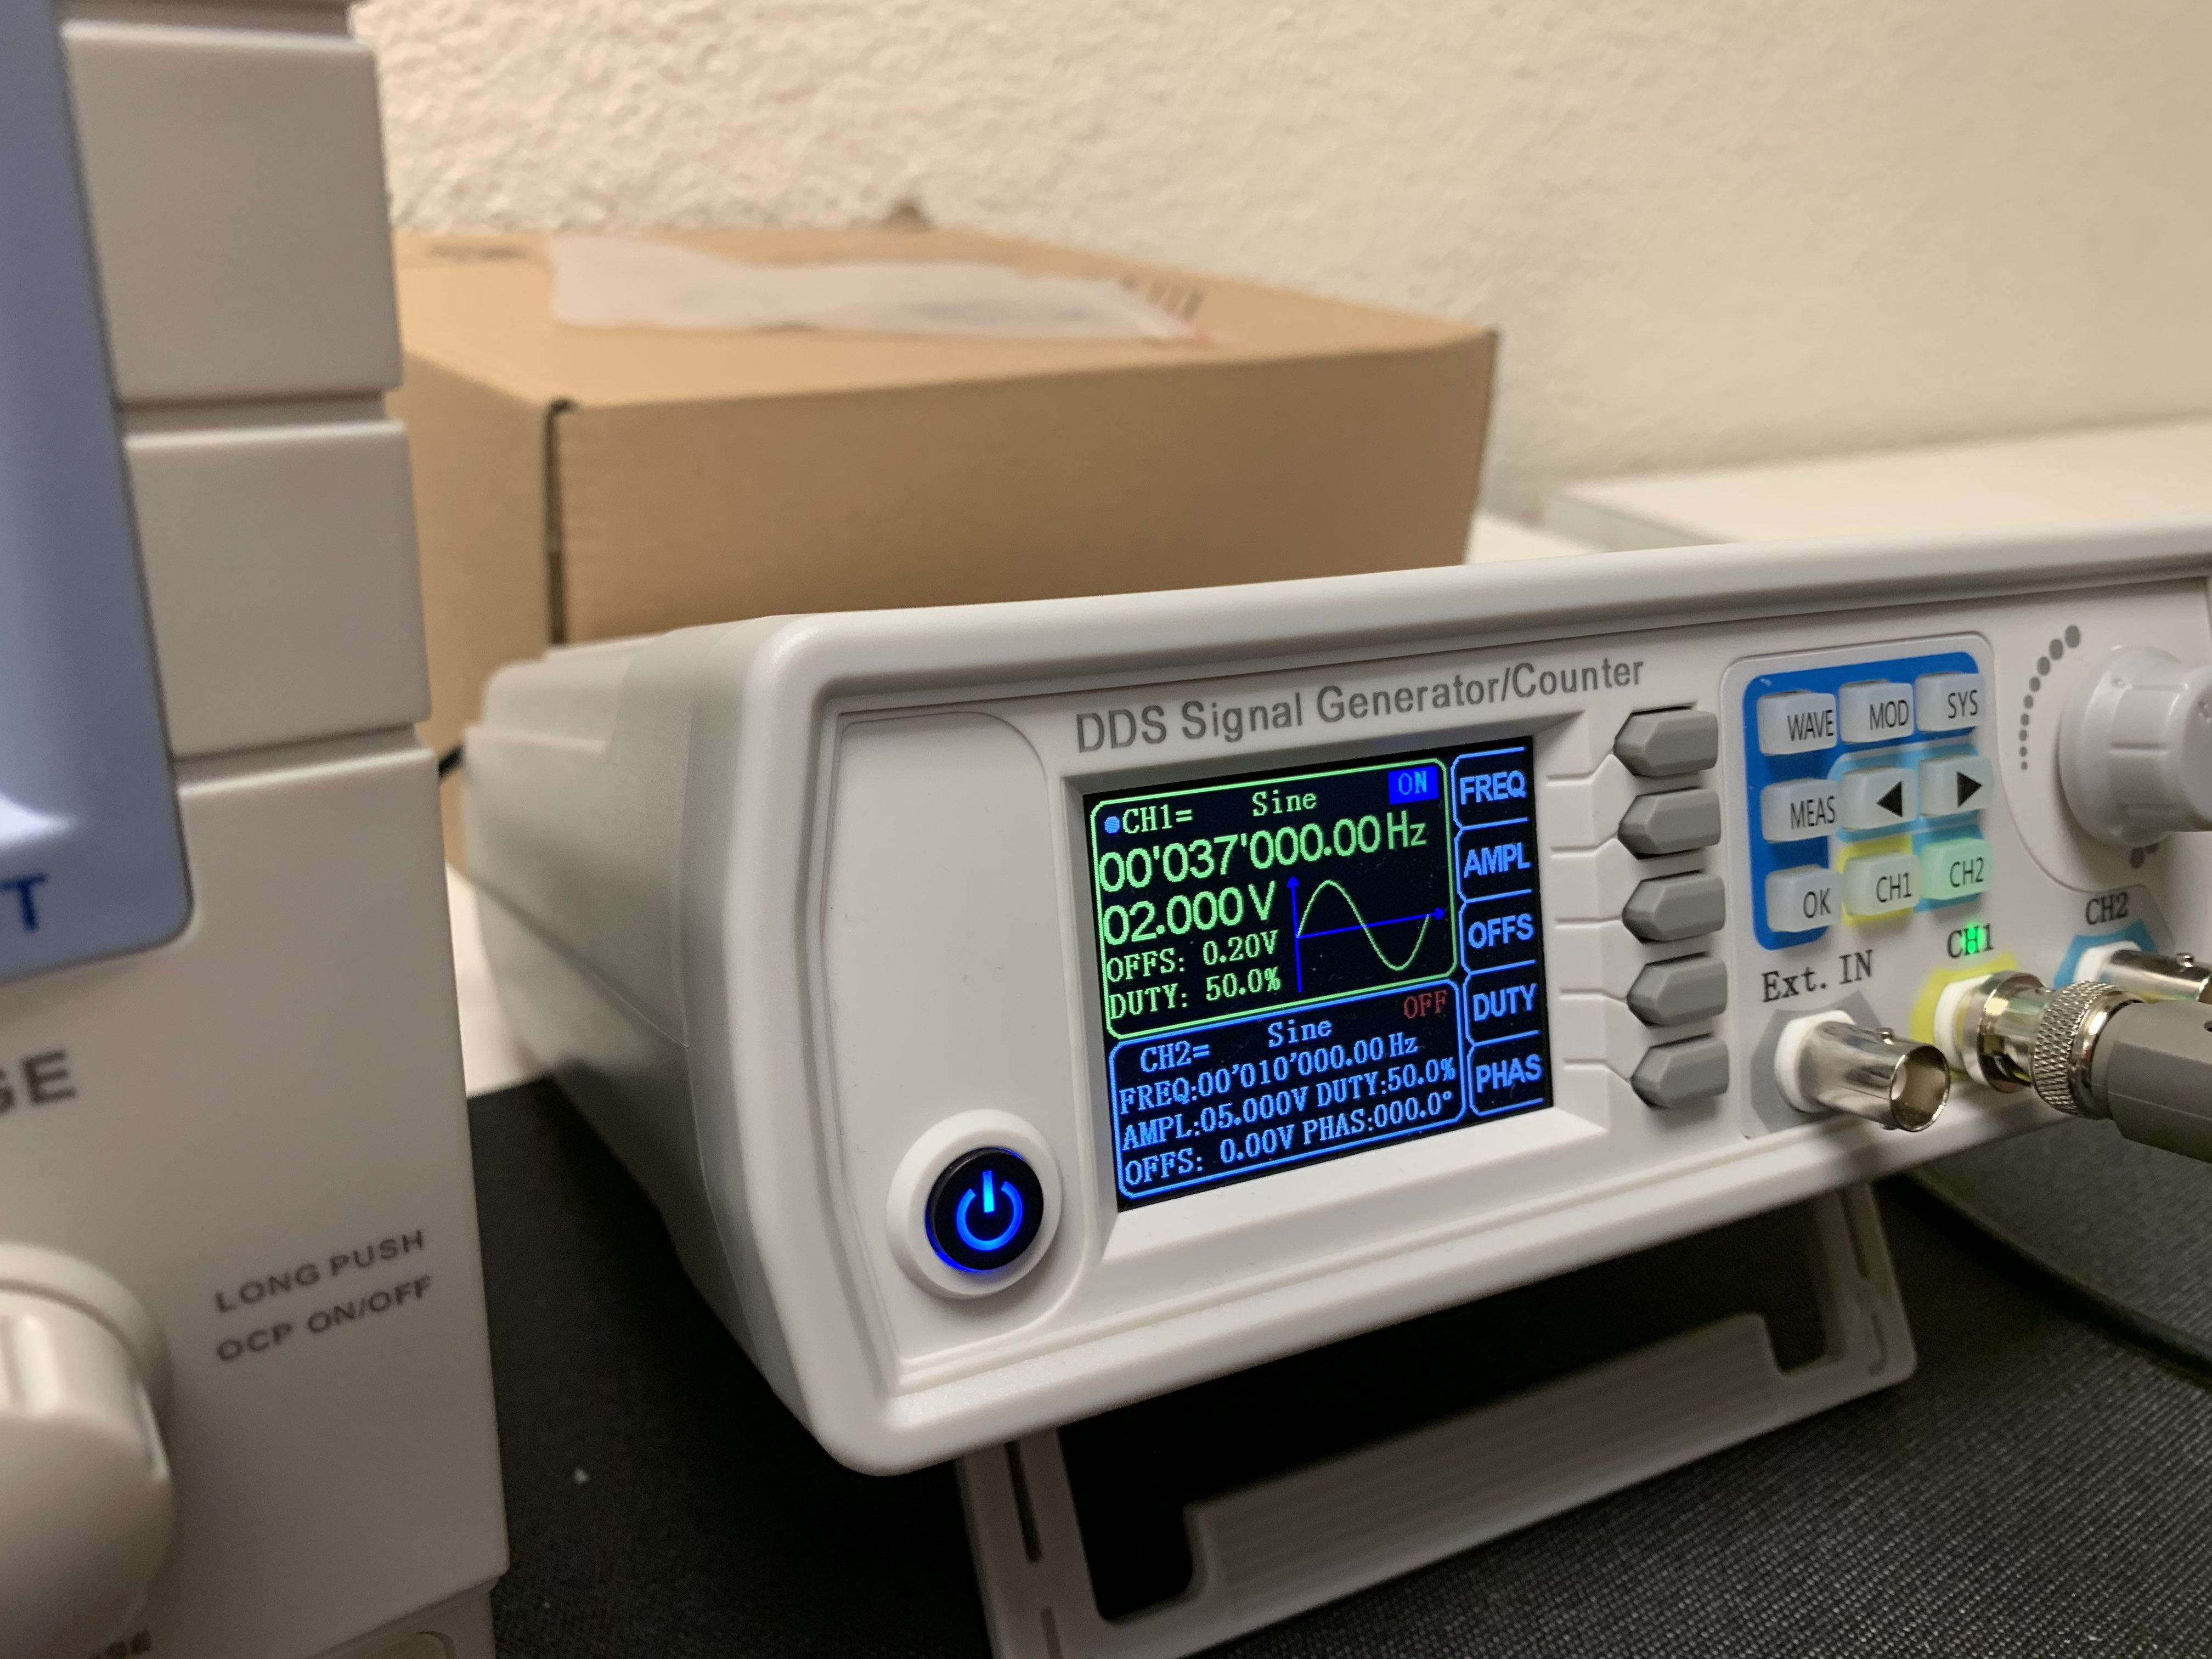
\includegraphics[scale=.05]{sin_func.jpg}\\
	\end{center}
	Set up the Signal generator to output a sin wave by cycling through the options with the "wave" button.\\

	\begin{center}
		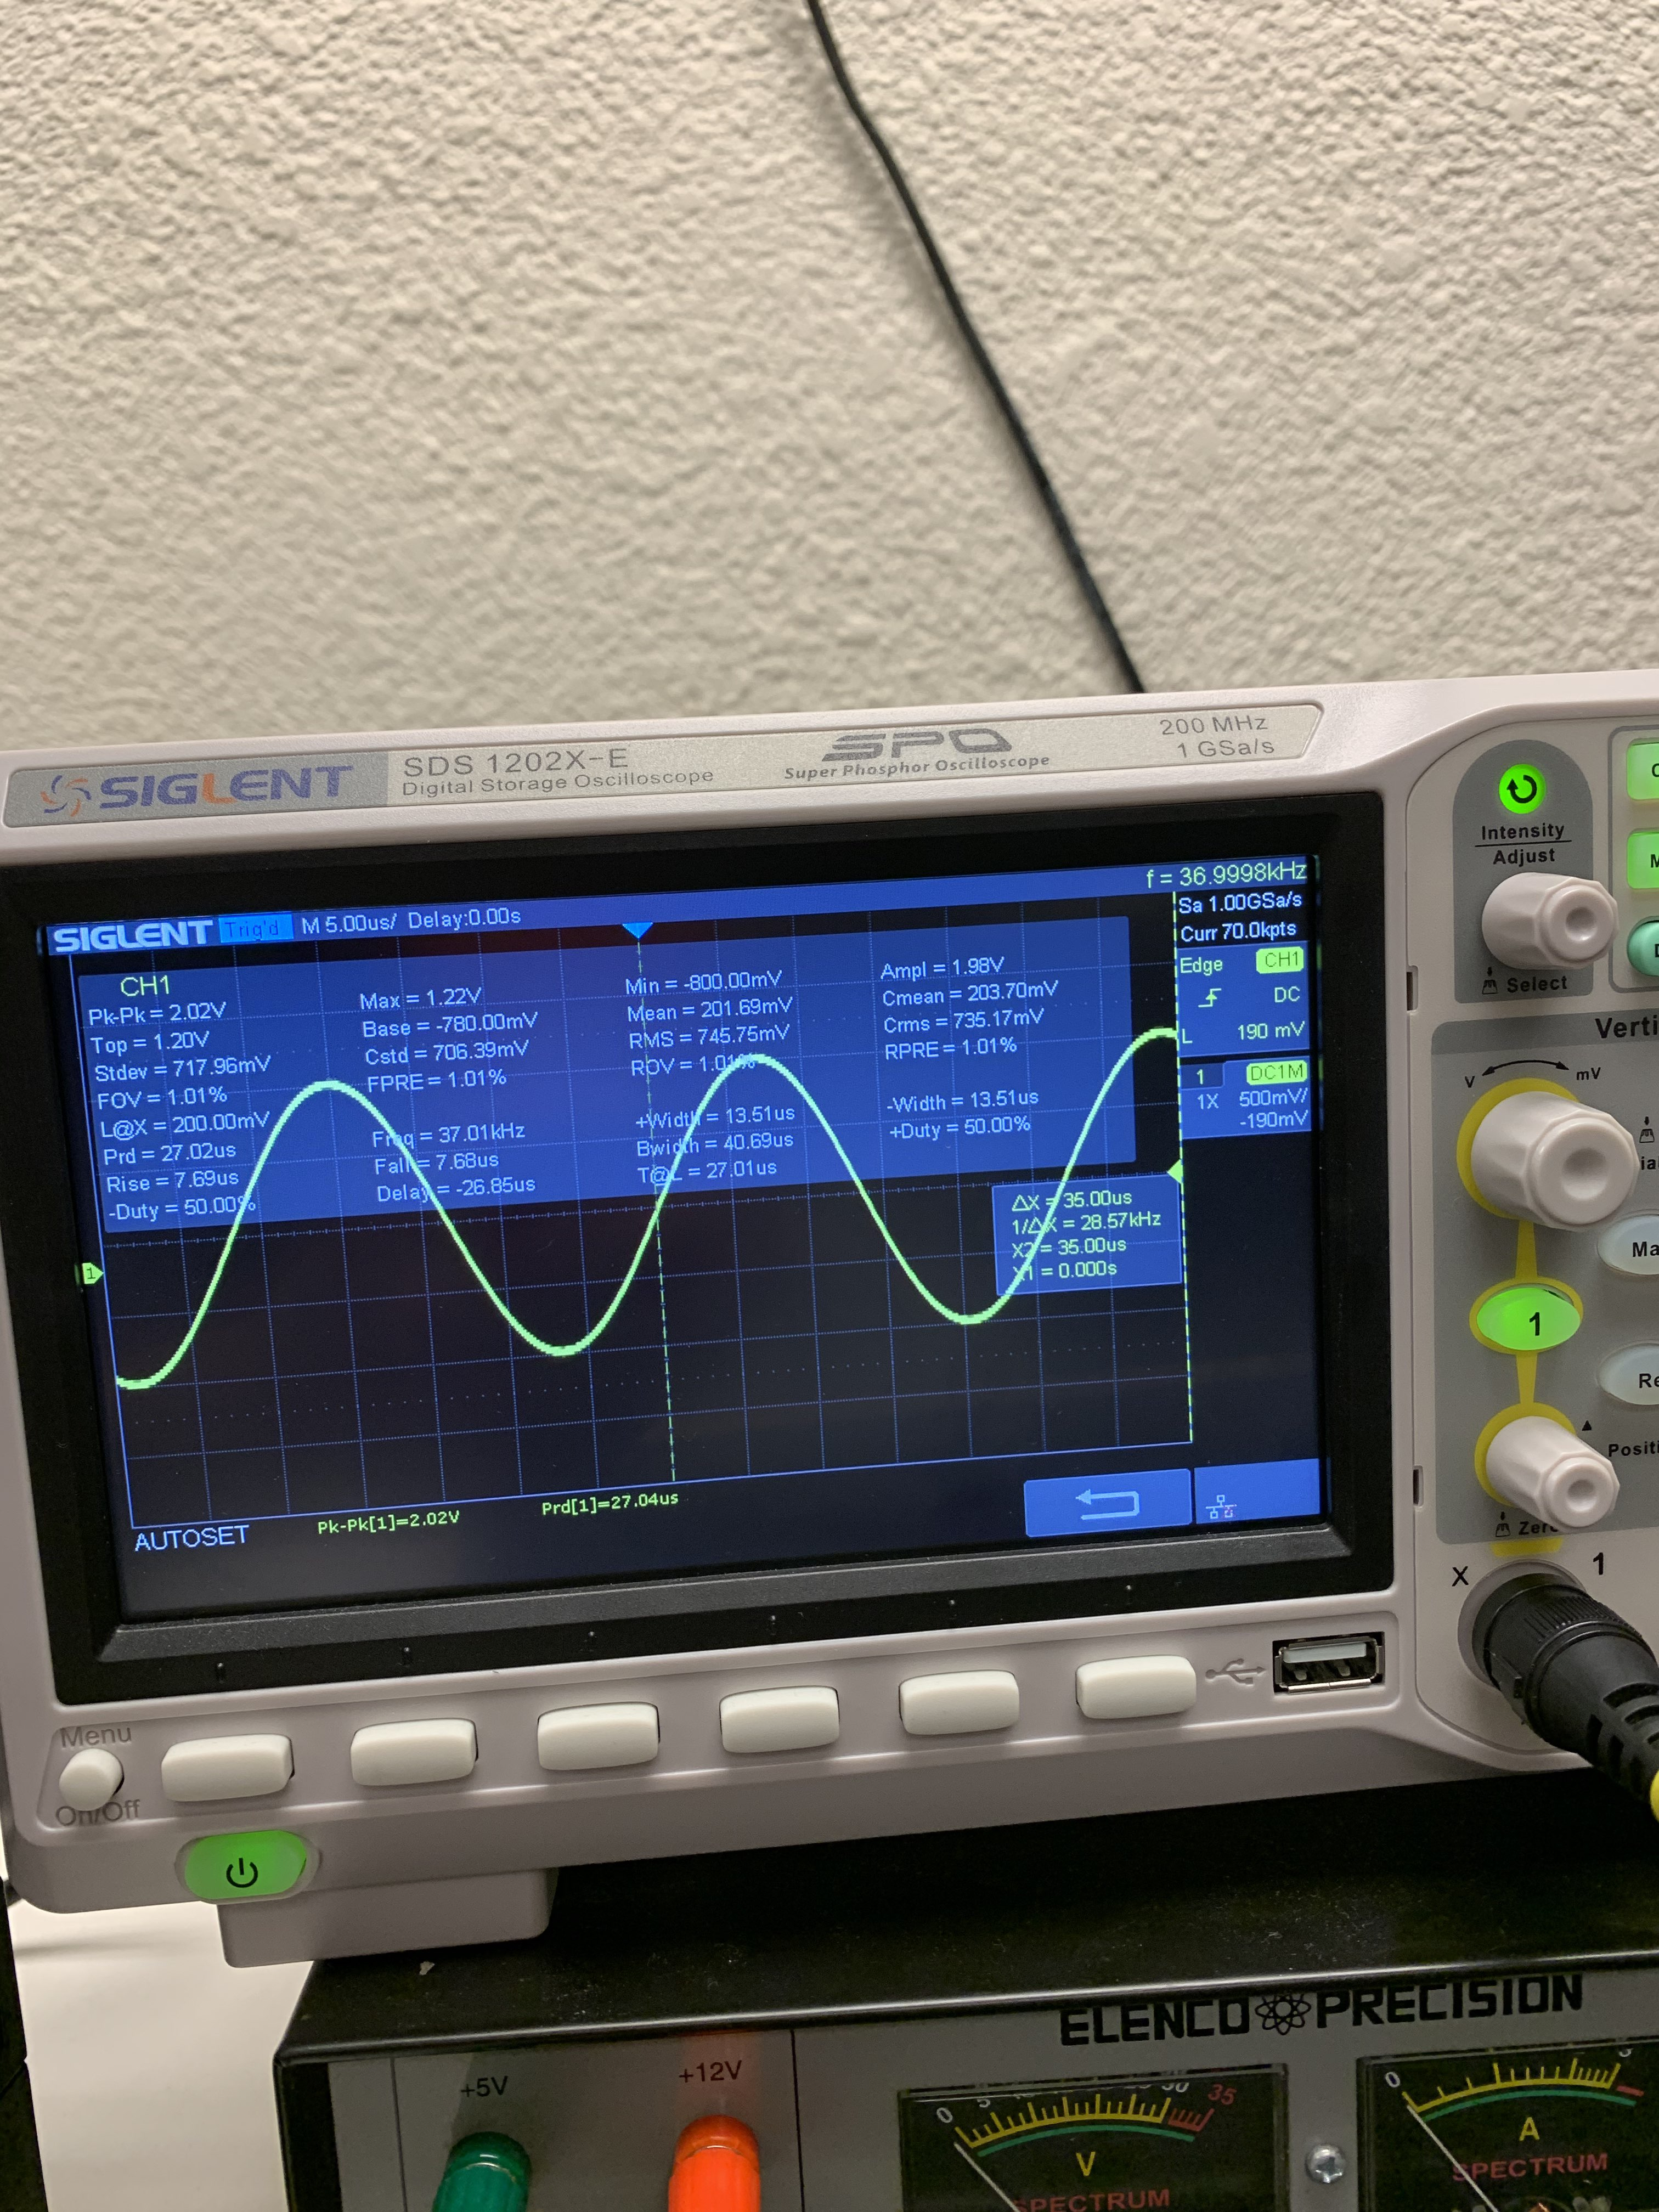
\includegraphics[scale=.05]{sin_osci.jpg}\\
	\end{center}
	This is how it appears on the Oscilloscope.

\section{Pulse Wave}
	\begin{center}
		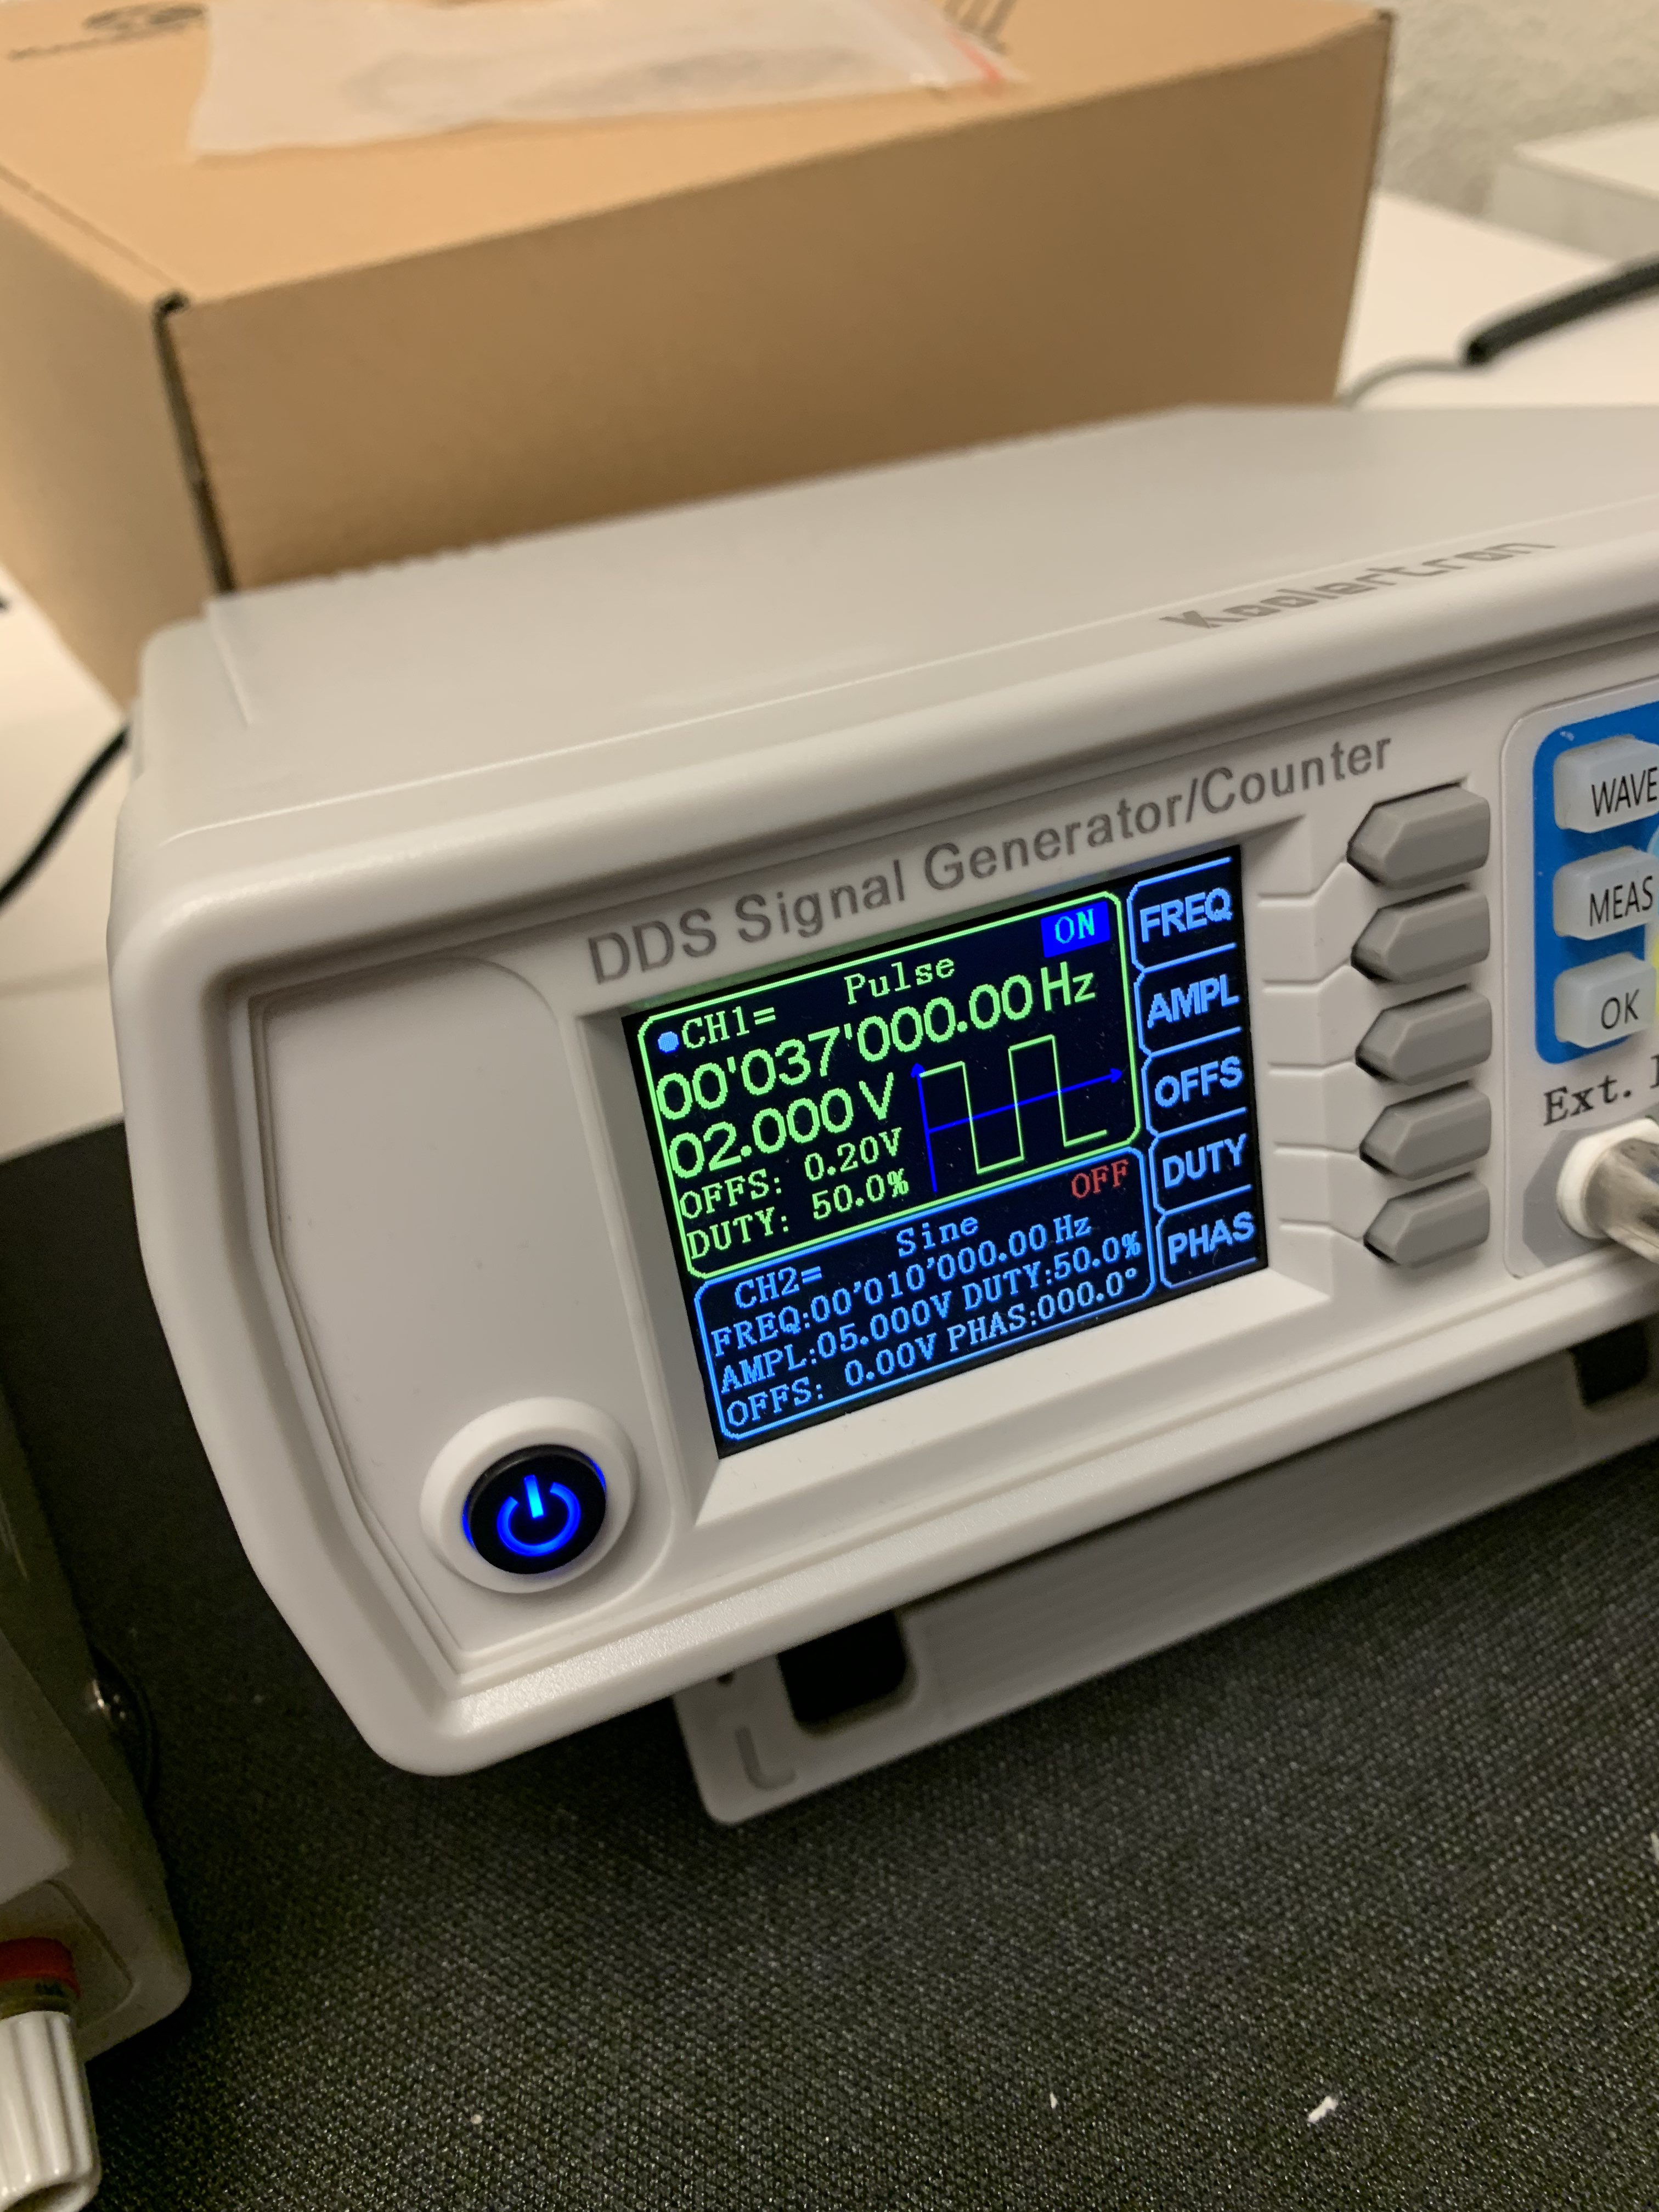
\includegraphics[scale=.05]{pulse_func.jpg}\\
	\end{center}
	Set up the Signal generator to output a pusle wave by cycling through the options with the "wave" button.\\

	\begin{center}
		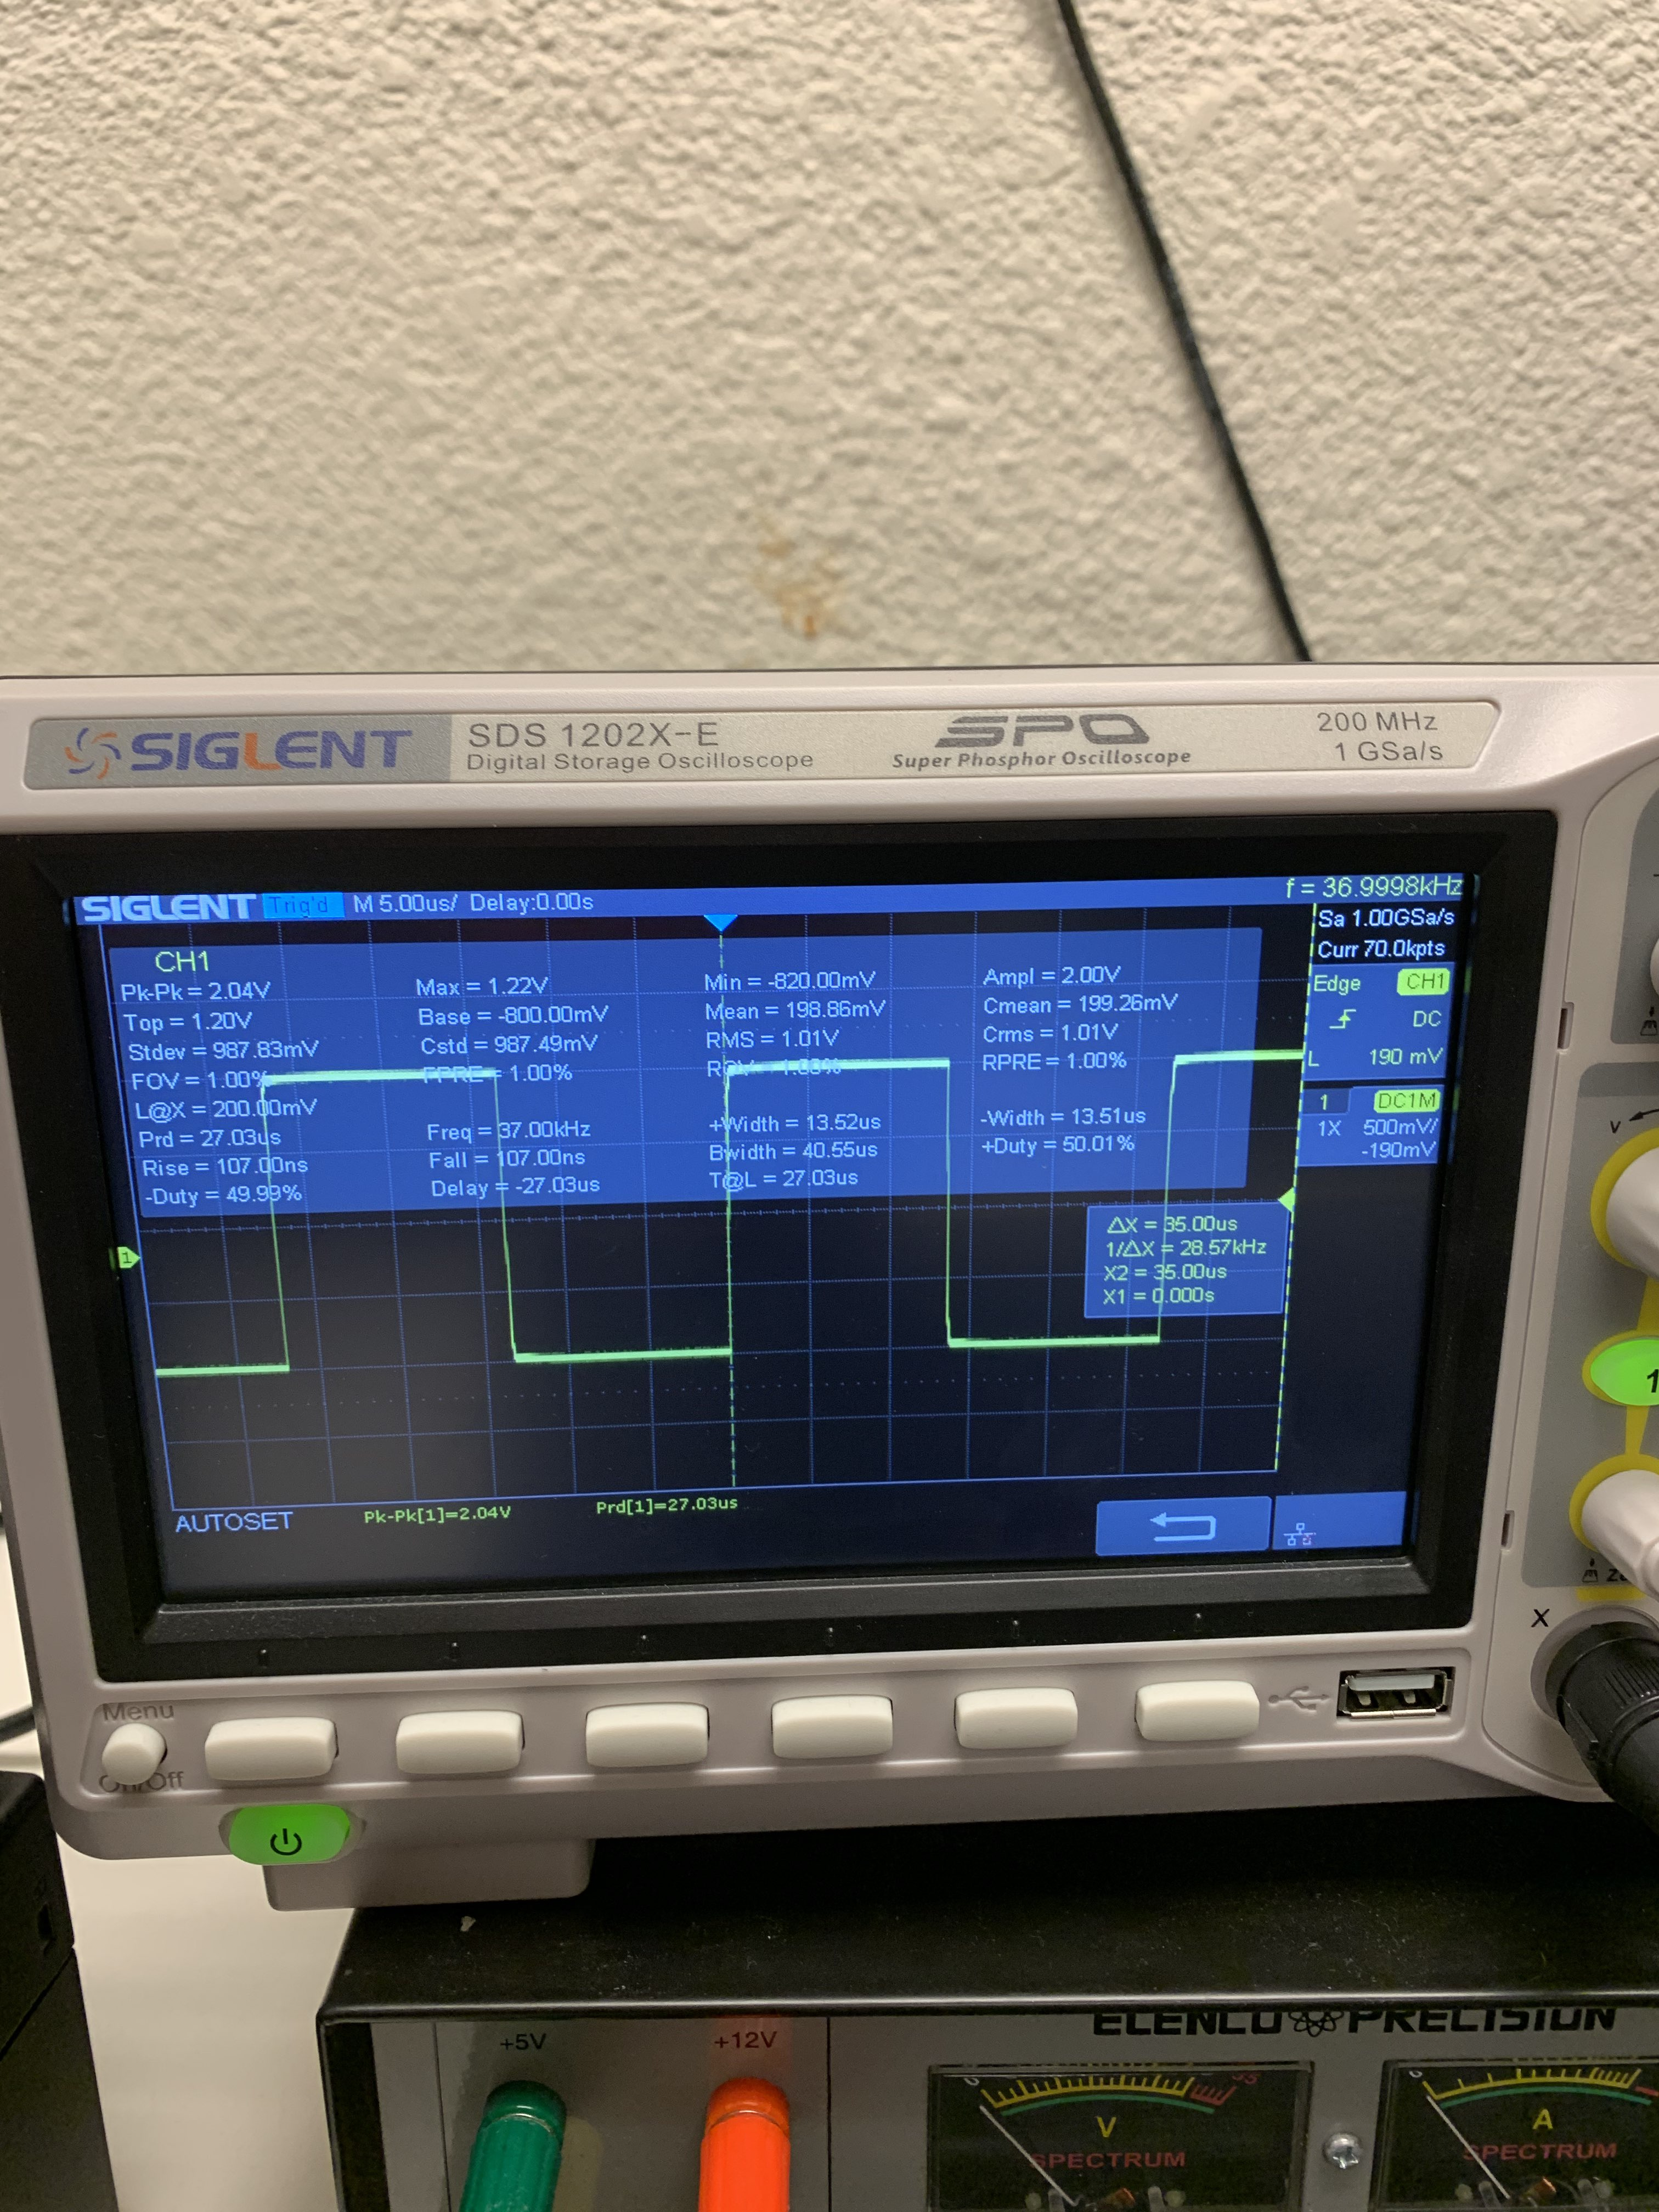
\includegraphics[scale=.05]{pulse_osci.jpg}\\
	\end{center}
	This is how it appears on the Oscilloscope.



\end{document}
